% Gerado por analises.rq01_04; nao editar manualmente.

A análise utiliza 300 repositórios, com peso igual por repositório. Valores ausentes são excluídos por métrica; zero é mantido. O IQR é Q3 menos Q1, com quantis por interpolação linear. A tabela mostra proporções de CFR, não percentuais.

\begin{table}[ht]\centering\small

\caption{RQ 01 a 04: estatísticas por repositório.}\label{tab:rq0104-resumo}

\begin{tabular}{lrrrrr}\hline Métrica & $n$ & Mediana & Q1 & Q3 & IQR \\ \hline

Frequência (releases/semana) & 300 & 0,518 & 0,249 & 1,208 & 0,959 \\

Lead time (a), h & 299 & 239,152 & 103,311 & 781,956 & 678,645 \\

Lead time (b), h & 299 & 263,645 & 96,999 & 893,543 & 796,544 \\

CFR (a) & 300 & 0,046 & 0,023 & 0,111 & 0,088 \\

CFR (b) & 298 & 0,181 & 0,022 & 0,400 & 0,378 \\

Recuperação, h & 285 & 2,621 & 1,029 & 6,829 & 5,801 \\

Fração censurada por repo & 288 & 0,001 & 0,000 & 0,019 & 0,019 \\

\hline\end{tabular}\end{table}

\begin{table}[ht]\centering\small

\caption{Distribuição C1: contagens, incluindo ausentes.}\label{tab:rq0104-c1}

\begin{tabular}{lrrrrr}\hline Métrica & Elite & High & Medium & Low & Ausentes \\ \hline

Frequência & 8 & 82 & 137 & 73 & 0 \\

Lead time (a) & 39 & 75 & 105 & 80 & 1 \\

CFR (a) & 249 & 34 & 10 & 7 & 0 \\

Recuperação & 71 & 182 & 31 & 1 & 15 \\

Geral C1 & 20 & 122 & 130 & 12 & 16 \\

\hline\end{tabular}\end{table}

C1 mantém as categorias de metrics.csv: releases, lead time (a), CFR (a) e recuperação de CI. A classificação geral usa a mediana das quatro notas, arredondada para baixo pelo pipeline; sem as quatro métricas, fica ausente. Essas faixas são as definições operacionais do estudo e não uma certificação de desempenho em produção.

\paragraph{RQ 01 e H1} A frequência mediana é 0,518 releases/semana; Q1=0,249, Q3=1,208, IQR=0,959 e máximo=49,556. A previsão de mediana abaixo de uma release por semana é compatível com os dados. Medium reúne 137/300 repositórios (45,7\%); não há maioria absoluta nessa categoria. Publicações automatizadas podem afetar a cauda, mas metrics.csv não permite testar essa explicação. Release é proxy de publicação, não evidência de deploy em produção.

\paragraph{RQ 02 e H2} As medianas são 239,152 h (a) e 263,645 h (b), com IQR 678,645 h e 796,544 h. Nos 299 pares válidos, (a) supera (b) em 178, empata em 1 e fica abaixo em 120; a mediana das diferenças pareadas é 24,491 h. A diferença entre medianas não substitui essa mediana pareada. Há 80 repositórios com (a) acima de 30 dias. A previsão de (b) na faixa High/Medium é compatível com sua mediana. A previsão de (a) maior não é compatível com a comparação das medianas agregadas; a maioria dos pares tem (a) maior. A leitura de H2 precisa separar distribuição agregada e comparação pareada, sem presumir que (a) seja sempre maior: (a) calcula o tempo do commit mais antigo até a publicação e depois a mediana entre releases; (b) agrega os tempos individuais dos commits, ponderando implicitamente releases com mais commits. Essa mudança de unidade e de ponderação pode inverter a comparação em alguns repositórios. A correlação exploratória entre frequência e diferença (a)-(b) é rho=-0,289, sem demonstrar causalidade. A duração de revisão de PRs e de branches não é observável nesse CSV.

\paragraph{RQ 03 e H3} O CFR mediano é 4,6\% no proxy de CI e 18,1\% no proxy de entrega; os IQRs são 8,8 e 37,8 pontos percentuais. A faixa prevista de 10\%-25\% para a mediana de CI não é observada. A previsão de mediana menor no proxy de entrega não é compatível com os dados. Dos 298 repositórios com CFR (b) válido, 139 ficam abaixo de 15\% e 71 têm zero. A correlação de Spearman entre os proxies é rho=0,126 em 298 pares (p exploratório=0,029039). São construtos diferentes: CI mede execuções elegíveis com falha; entrega procura uma release corretiva em até sete dias. Uma falha de teste, lint ou dependência externa não comprova incidente em produção. Uma correção publicada pode estar ligada a mudança anterior. Releases sem sete dias completos de acompanhamento são censuradas, não tratadas como sucesso. A magnitude do rho é a evidência para a expectativa de associação fraca em H3; um p pequeno não implica correlação forte nem equivalência entre os proxies.

\paragraph{RQ 04 e H4} A mediana entre as medianas de recuperação dos repositórios é 2,621 h, com Q1=1,029, Q3=6,829, IQR=5,801 e máximo=181,768 h. A expectativa de mediana entre uma hora e um dia é compatível com o resultado. Há 147 repositórios com algum episódio censurado, 12 sem episódios e 3 somente com episódios censurados. No agregado ponderado por episódios, são 307/64677 (0,47\%). Essa razão não é a mediana das proporções por repositório. A tabela de censura lista ambos os contadores e a proporção para cada repositório. O tempo considera apenas episódios recuperados no mesmo workflow; censurados são excluídos das durações e podem subestimar tempos longos. Não estimamos a distribuição de sobrevivência dos episódios a partir dessas medianas agregadas. A relação com workflows auxiliares prevista em H4 não pode ser testada apenas com metrics.csv.

\begin{figure}[ht]\centering

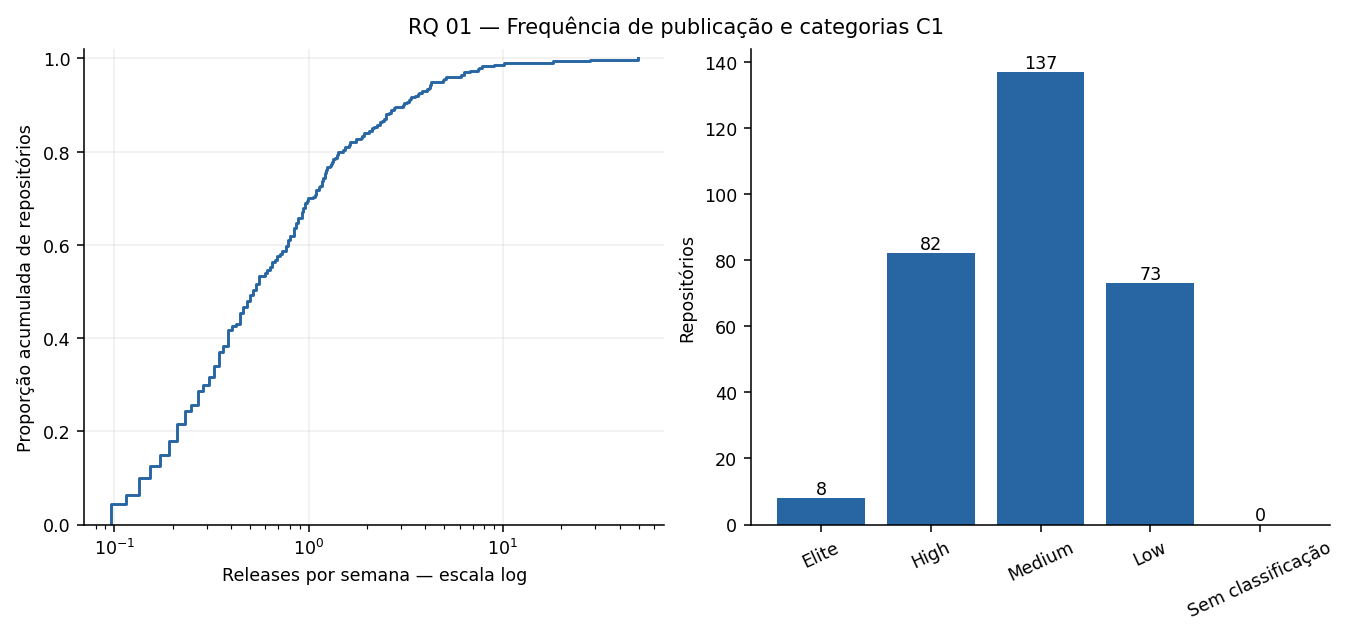
\includegraphics[width=\linewidth]{figuras/rq01_frequencia.png}

\caption{Frequência de publicação e categorias C1.}\label{fig:rq0104-rq01-frequencia}

\end{figure}

\begin{figure}[ht]\centering

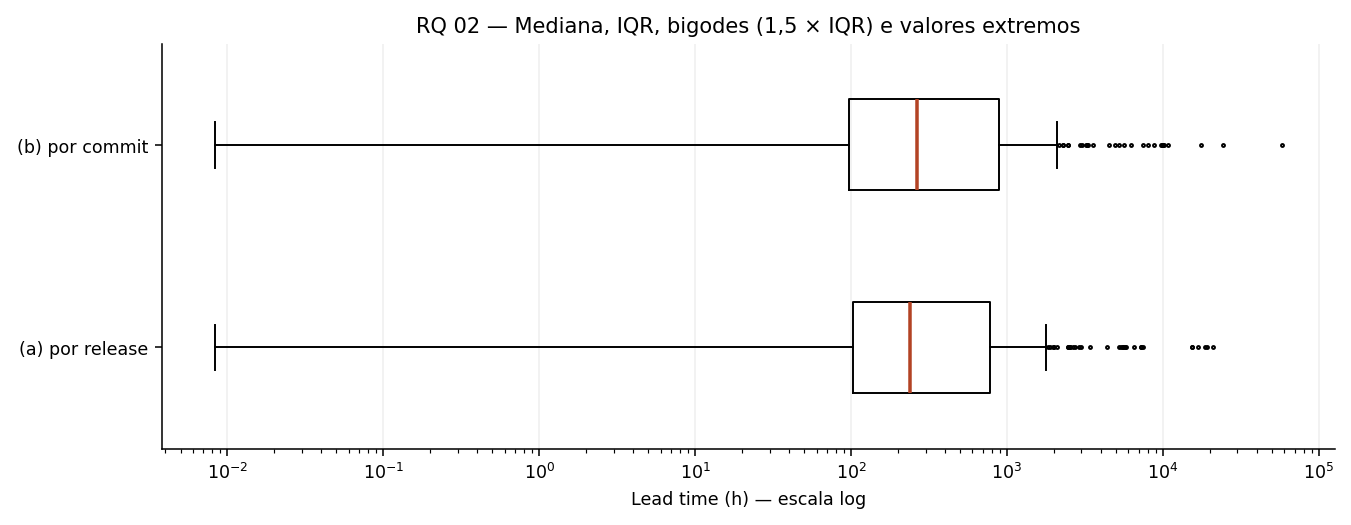
\includegraphics[width=\linewidth]{figuras/rq02_lead_time.png}

\caption{Lead time nas duas variantes.}\label{fig:rq0104-rq02-lead-time}

\end{figure}

\begin{figure}[ht]\centering

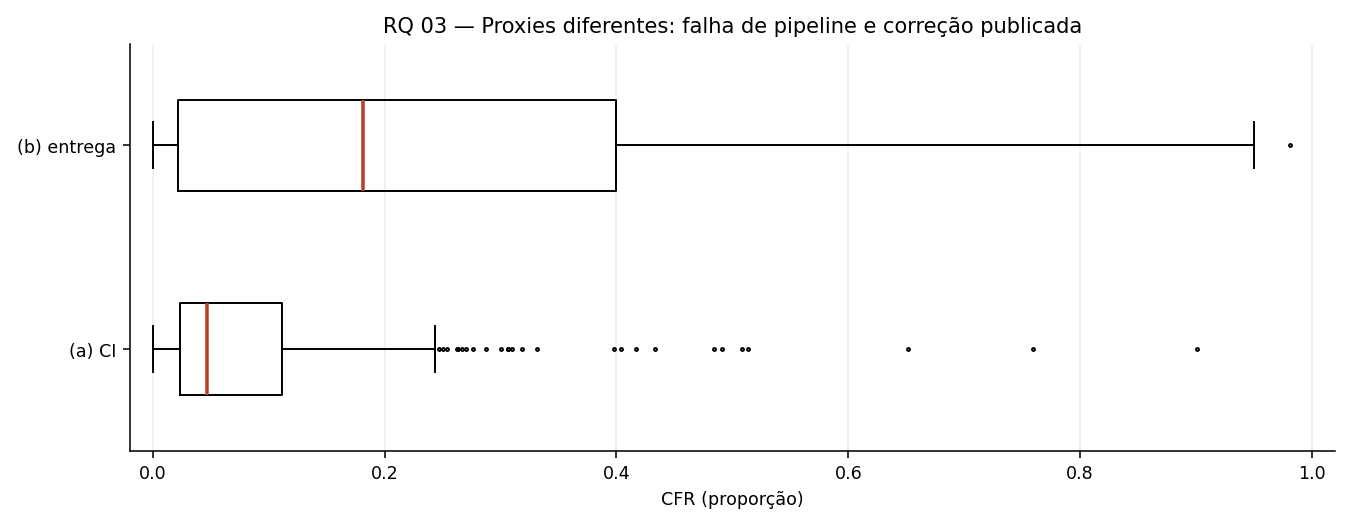
\includegraphics[width=\linewidth]{figuras/rq03_cfr.png}

\caption{CFR de CI e de entrega.}\label{fig:rq0104-rq03-cfr}

\end{figure}

\begin{figure}[ht]\centering

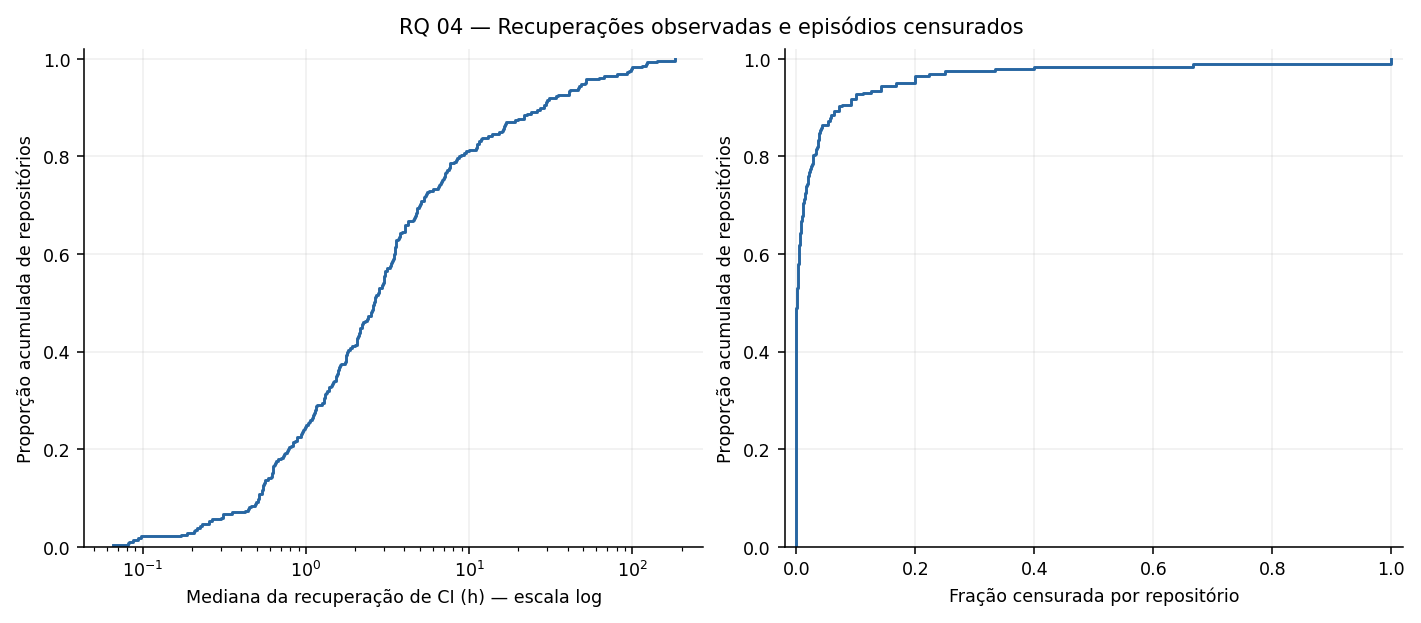
\includegraphics[width=\linewidth]{figuras/rq04_recuperacao.png}

\caption{Recuperação observada e proporções censuradas.}\label{fig:rq0104-rq04-recuperacao}

\end{figure}

\begin{figure}[ht]\centering

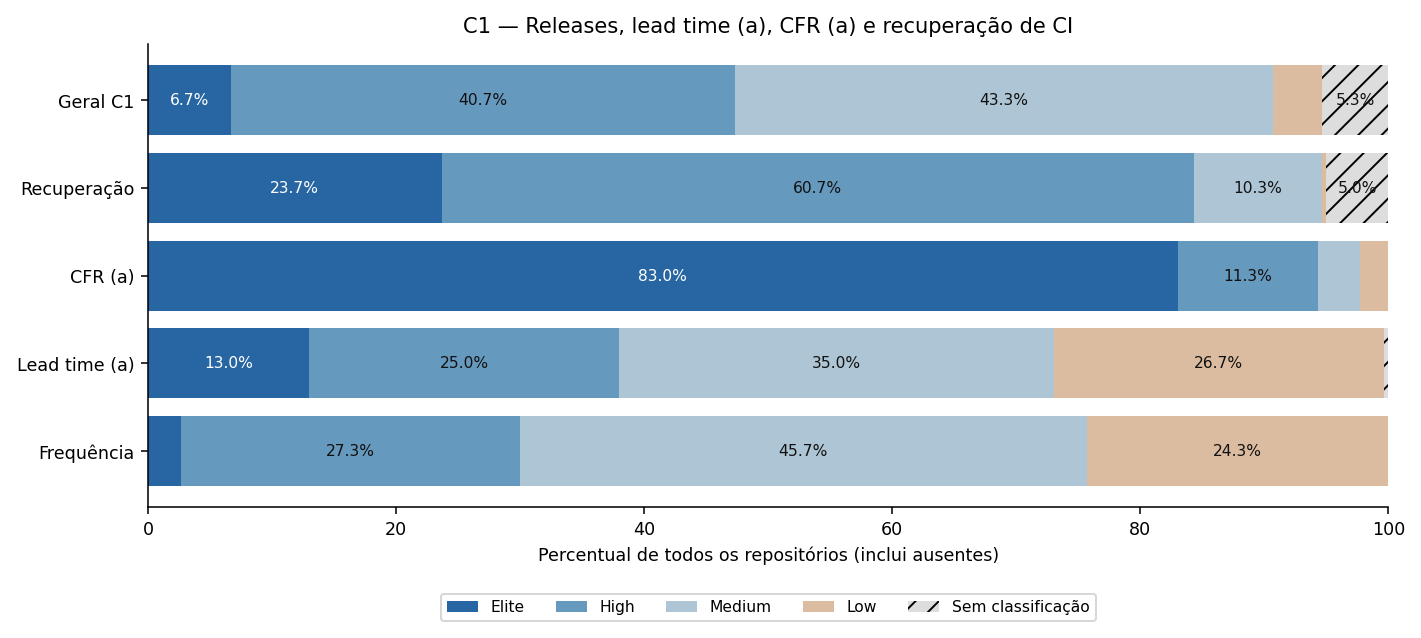
\includegraphics[width=\linewidth]{figuras/c1_categorias.png}

\caption{Categorias C1 por métrica e geral.}\label{fig:rq0104-c1-categorias}

\end{figure}
